
\section{The \pkg{sbtools} package}
\begin{itemize}
	\item{Goal to allow programmatic access to core SB functionality}
	\item{Harmonize the SB data structures with common R interfaces}
	\item{Lightweight R package that can be quickly added to existing projects and shared broadly}
\end{itemize}


%code example
% \begin{example}
  % x <- 1:10
  % result <- myFunction(x)
% \end{example}

\subsection{Data access API}
The data access functionality of \pkg{sbtools} makes it easy to 
access any public item's data, attached files and metadata. All items
in ScienceBase have a unique identifier that can be used to directly 
access specific items. 

\begin{example}
> test_item = item_get("4f4e4b24e4b07f02db6aea14")
> test_item
<ScienceBase Item> 
  Title: Coastal-change and glaciological maps of Antarctica
  Creator/LastUpdatedBy:      / 
  Provenance (Created / Updated):  2010-10-06T04:25:43Z / 2014-07-21T17:45:42Z
  Children: FALSE
  Item ID: 4f4e4b24e4b07f02db6aea14
  Parent ID: 4f4e4771e4b07f02db47e1e4
\end{example}

For convenience, \pkg{sbtools} defines an \code{sbitem} object, which is 
returned by \pkg{sbtools} functions when referencing objects. The underlying
data structure is a list. All available metadata for an item can be listed
and accessed in the same way as a named list.

\begin{example}
> names(test_item) 
 [1] "link"              "relatedItems"      "id"               
 [4] "identifiers"       "title"             "citation"         
 [7] "provenance"        "hasChildren"       "parentId"         
[10] "contacts"          "webLinks"          "browseCategories" 
[13] "browseTypes"       "tags"              "dates"            
[16] "facets"            "files"             "distributionLinks"
[19] "previewImage"     

> item_get(test_item)$citation
[1] "Geological Survey (U.S.), 1999-08-05, Coastal-change 
and glaciological maps of Antarctica:  Fact SheetCoastal-change and 
glaciological maps of Antarctica."
\end{example}

On ScienceBase, all items are organized in a tree structure, with one 
parent and potentially many children. \pkg{sbtools} allows the user to 
easily traverse the tree structure. For example, in some projects, the hierarchy has 
important meaning. For other projects, it may relates to the user or
organizational owner of the data.

\begin{example}
#parent ID always available as item attribute
> parent = item_get(test_item$parentId)
> parent
  Title: USGS Publications Warehouse
  Creator/LastUpdatedBy:      / 
  Provenance (Created / Updated):  2012-02-29T15:42:41Z / 2014-07-08T21:42:20Z
  Children: TRUE
  Item ID: 4f4e4771e4b07f02db47e1e4
  Parent ID: 4f4e4771e4b07f02db47e1da
  
#getting sibling items
> item_list_children(parent)
[1] "55b98fbee4b08f6647be5179" "541d45a4e4b0f68901ec30ef"
[3] "55b361b3e4b09a3b01b5daad" "53516ef9e4b05569d8059f34"
[5] "4f4e4ab2e4b07f02db66f5e3" "5351704ee4b05569d805a2e4"
\end{example}

ScienceBase items may have data or metadata files attached to them. 
You can list and download attached files directly using \pkg{sbtools}.

\begin{example}
#returns files attached to item
item_list_files(test_item)
#returns local path to downloaded files
item_file_download(test_item, dest_dir = tempdir())
\end{example}

ScienceBase has special functionality when certain data types are 
stored. One example is spatial data. When spatial data are properly 
tagged and uploaded to ScienceBase, they can be accessed using OGC 
web services. \pkg{sbtools} has included ability to access the Web
Feature Service (WFS) available for certain items.

\begin{example}
#Source non-sbtools-required but useful mapping packages
library(maps)
library(sp)
#an item with an included OGC WFS service
layer = item_get_wfs('55e372b9e4b05561fa208212')
map('state', regions='iowa')
plot(layer, add=TRUE)
\end{example}

%this figure code is demo\figure_map_code.R 
% feel free to improve
 \begin{figure}[htbp]
   \centering
   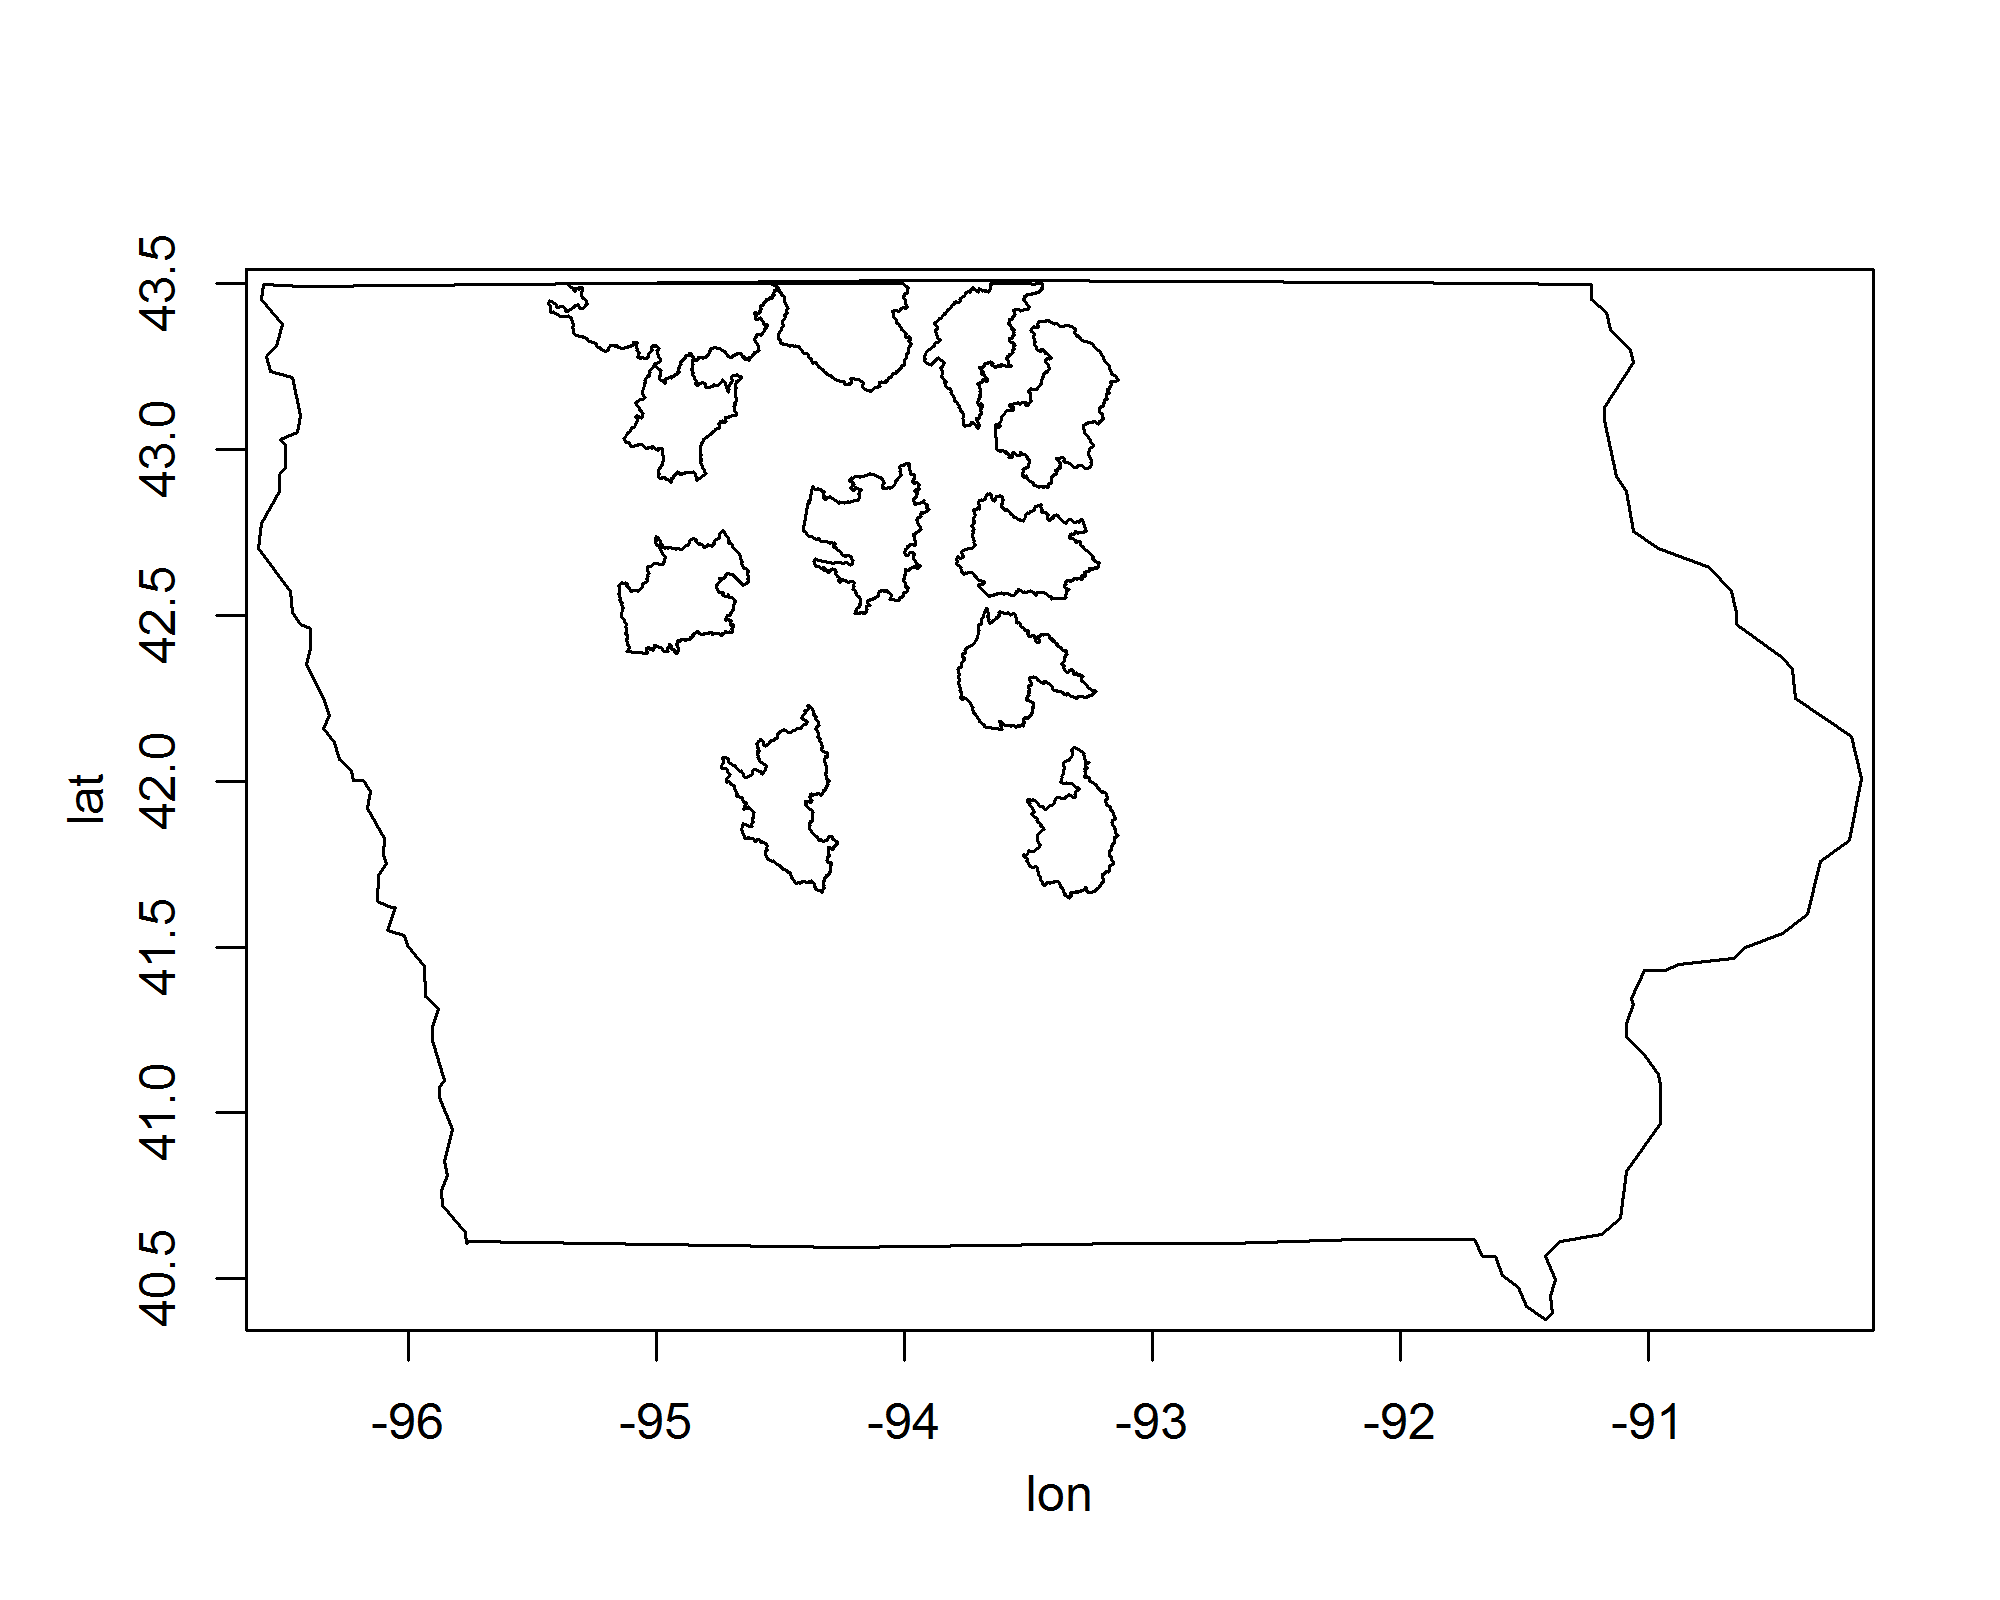
\includegraphics{mapfig}
   \caption{An example spatial dataset from ScienceBase, 
   visualized on top of the outline for the state of Iowa}
   \label{figure:iowafig}
 \end{figure}


\subsection{Search API}
\begin{itemize}
	\item{Go over general search API}
	\item{Free text search}
	\item{dateRange query}
	\item{Spatial query}
	\item{Hierarchical SB queries (sub-items)}
	\item{Combination of above}
\end{itemize}

\subsection{ScienceBase authenticated}
ScienceBase has a large collection of open, reusable datasets and 
useful metadata. In addition to the public data available, ScienceBase
is also a platform for sharing and collaboration on private or in-progress 
data accessible through authenticated sessions. \pkg{sbtools} supports 
authentication to interact with access controlled items.

Authentication in \pkg{sbtools} is handled through the persistence of 
an authenticated session. By storing only the session, we do not need to 
store the plaintext password, which could represent a security issue. This
session state is persisted between function calls by the package. While  
expiration of the session can be difficult to predict, \pkg{sbtools}
makes a best effort to supply the user with meaningful error messages.

The authentication function \code{authenticate_sb} can accept a username
and password. Alternatively, to prevent plaintext passwords in R history, 
the password can be omitted and will be requested by R interactively. 
Authentication is persisted by the package, allowing for a single sign-in
and no tracking of usernames, passwords, or sessions during interactive or
script-based use. 

%Examples of authentication and other auth-related functions (check and such)
\begin{example}



\end{example}

\begin{itemize}
	\item{How authentication changes SB}
	\item{Authentication in sbtools}
	\item{Authentication persistence and use throughout package}
	\item{Examples of authentication and other auth-related functions (check and such)}
\end{itemize}

\subsection{Data editing and upload API}
This will be an extensive section
\begin{itemize}
	\item{Item creation}
	\item{Item deletion}
	\item{Attached file upload, replacement and deletion}
	\item{}
\end{itemize}

\subsection{SB Item identifiers}
\begin{itemize}
	\item{Functionality of item identifiers}
	\item{Example of identifier use}
	\item{How identifiers can be useful for projects}
\end{itemize}
